%DLG
\section{Introduction}
%%%%%%%%%%%%%%%%%%%%% IN SHORT: the background of distributed training and collaborative learning
Distributed training becomes necessary to speedup training on large-scale datasets.
In a distributed learning system, the computation is executed parallely on each worker and synchronized via exchanging gradients (both parameter server~\cite{li2014scaling, iandola2016firecaffe} and all-reduce~\cite{barney2010introduction_to_parallel_computing, patarasuk2009ring_all_reduce}).
The distribution of computation naturally leads to the splitting of data: 
Each client has its own the training data and only communicates gradient during training (says the training set never leaves local machine). 
It allows to train a model using data from multiple sources without centralizing them. This scheme is named as collaborative learning and widely used when the training set contains private information~\cite{jochems2016distributed, google2016federated}. For example, multiple hospitals train a model jointly without sharing their patients' medical data~\cite{jochems2017developing, mcmahan2016communication}. 

%%%%%%%%%%%%%%%%%%%%% IN SHORT: Put the question and shows our results
Distributed training and collaborative learning have been widely used in large scale machine learning tasks. However, \textbf{does the ``gradient sharing'' scheme protect the privacy of the training datasets of each participant?} 
In most scenarios, people assume that gradients are safe to share and will not expose the training data. Some recent studies show that gradients reveal some properties of the training data, for example, property classifier~\cite{Melis2018unintended} (whether a sample with certain property is in the batch) and using generative adversarial networks to generate pictures that look similar to the training images~\cite{hitaj2017information, Melis2018unintended, fredrikson2015model_inversion}. 
Here we consider a more challenging case: can we \textbf{completely} steal the training data from gradients? 
Formally, given a machine learning model $F()$ and its weights $W$, if we have the gradients $\nabla w$ w.r.t a pair of input and label, can we obtain the training data reversely? 
Conventional wisdom suggests that the answer is no, but we show that this is actually possible. 

%%%%%%%%%%%%%%%%%%%%% IN SHORT: Introduce our algorithms
In this work, we demonstrate \emph{Deep Leakage from Gradients} (\textbf{DLG}): 
sharing the gradients can leak private training data.
We present an optimization algorithm that can obtain both the training inputs and the labels in just few iterations. To perform the attack, we first randomly generate a pair of ``dummy'' inputs and labels and then perform the usual forward and backward. After deriving the dummy gradients from the dummy data, instead of optimizing model weights as in typical training, we optimize the dummy inputs and labels to minimize the distance between dummy gradients and real gradients (illustrated in Fig.~\ref{fig:methods}).
Matching the gradients makes the dummy data close to the original ones (Fig.~\ref{fig:vision_fig3}). 
When the optimization finishes, the private training data (both inputs and labels) will be fully revealed.
% Notably, the whole process requires no prior about the training set. 

%%%%%%%%%%%%%%%%%%%%%%%%%%%%%%%%%%%%%%%%%%%%%%%%%
% Attack Scenario
% Experiment Results
% Defense Strategy
%%%%%%%%%%%%%%%%%%%%%%%%%%%%%%%%%%%%%%%%%%%%%%%%%
% Advantage over conventional attack methods and attack results
Conventional ``shallow'' leakages (property inference~\cite{shokri2017membership, Melis2018unintended} and generative model~\cite{hitaj2017information} using class labels) requires extra label information and can only generate similar synthetic images. 
Our ``deep'' leakage is an optimization process and does not depend on any generative models; therefore, DLG does not require any other extra prior about the training set, instead, it can infer the label from shared gradients and the results produced by DLG (both images and texts) are the exact original training samples instead of synthetic look-alike alternatives.
% 
We evaluate the effectiveness of our algorithm on both vision (image classification) and language tasks (masked language model). On various datasets and tasks, DLG fully recovers the training data in just a few gradient steps. 
% 
Such a deep leakage from gradients is first discovered and we want to raise people's awareness of rethinking the safety of gradients. 

% Attack scenario and defense results
The deep leakage puts a severe challenge to the multi-node machine learning system. 
% 
The fundamental gradient sharing scheme, as shown in our work, is not always reliable to protect the privacy of the training data.  
% 
In centralized distributed training (Fig.~\ref{fig:overview:left}), the parameter server, which usually does not store any training data, is able to steal local training data of all participants. For decentralized distributed training (Fig.~\ref{fig:overview:right}), it becomes even worse since any participant can steal its neighbors' private training data.
% 
To prevent the deep leakage, we demonstrate three defense strategies: gradient perturbation, low precision, and gradient compression. For gradient perturbation, we find both Gaussian and Laplacian noise with a scale higher than $10^{-2}$ would be a good defense. While half precision fails to protect, gradient compression successfully defends the attack with the pruned gradient is more than 20\%.

\begin{figure}
    \centering
    \begin{subfigure}[b]{0.53\textwidth}
        \centering
        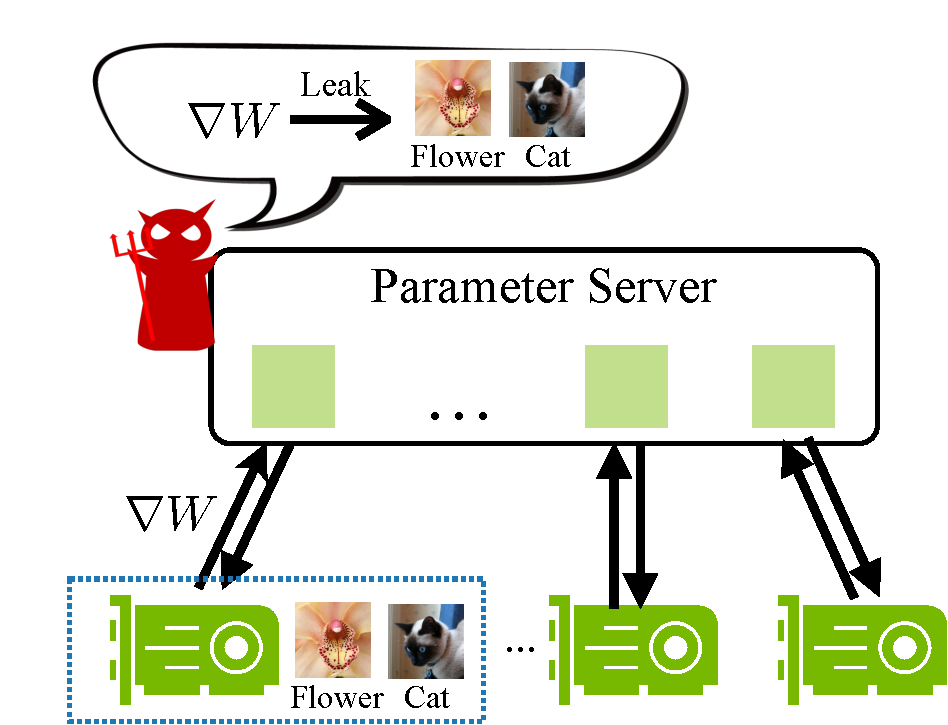
\includegraphics[width=\textwidth]{figures/fig1_left-crop.pdf}
        \caption{Distributed training with a centralized server}
        \label{fig:overview:left}
    \end{subfigure}
    \begin{subfigure}[b]{0.46\textwidth}
        \centering
        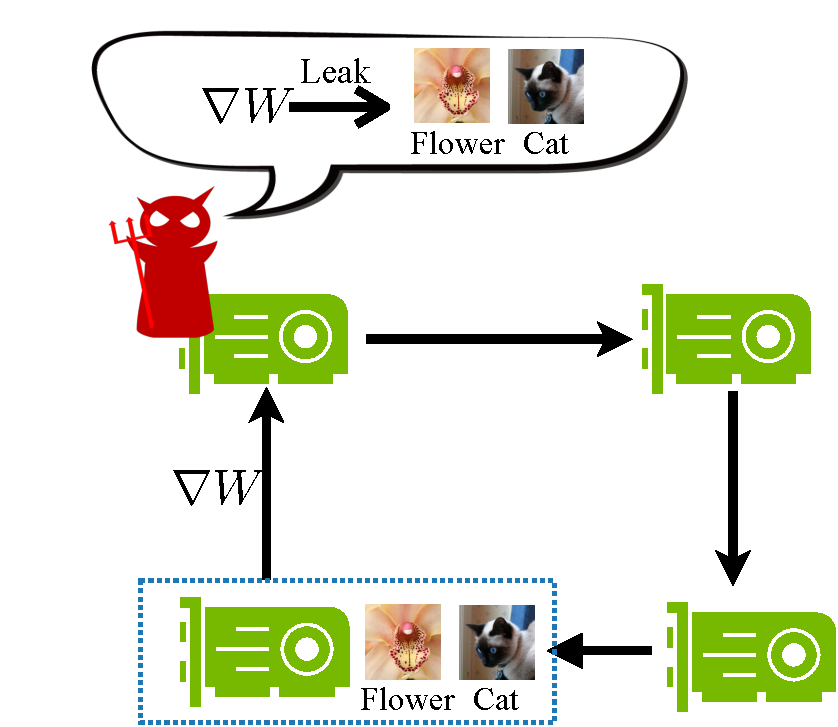
\includegraphics[width=\textwidth]{figures/fig1_right-crop.pdf}
        \caption{Distributed training without a centralized server}
        \label{fig:overview:right}
    \end{subfigure}
    \caption{The deep leakage scenarios in two categories of classical multi-node training. The little red demon appears in the location where the deep leakage might happen.   When performing centralized training, the parameter server is capable to steal all training data  from gradients received from worker nodes. While training in a decentralized manner (e.g., ring all reduce~\cite{patarasuk2009ring_all_reduce}), any participant can be malicious and steal the training data from its neighbors.}
    \label{fig:overview}
\end{figure}

Our contributions include:

\begin{itemize}
    \item We demonstrate that it is possible to obtain the private training data from the publicly shared gradients. To our best knowledge, DLG is the first algorithm achieving it. 
    \item DLG only requires the gradients and can reveal pixel-wise accurate images and token-wise matching texts. While conventional approaches usually need extra information to attack and only produce partial properties or synthetic alternatives. 
    \item To prevent potential leakage of important data, we analyze the attack difficulties in various settings and discuss several defense strategies against the attack.
\end{itemize}


